\documentclass[12pt]{article}

\usepackage[utf8]{inputenc}
\usepackage{amsmath,amssymb,hyperref,array,xcolor,multicol,verbatim,mathpazo}
\usepackage[normalem]{ulem}
\usepackage[pdftex]{graphicx}
\usepackage{fullpage}

\usepackage{threeparttable}
\usepackage{geometry}
\usepackage[format=hang,font=normalsize,labelfont=bf]{caption}
\usepackage{lscape}
\usepackage{natbib}
\usepackage{setspace}
\usepackage{float,color}
\usepackage[pdftex]{graphicx}
\usepackage{pdfsync}
\usepackage{placeins}
\usepackage{geometry}
\usepackage{pdflscape}
\usepackage[normalem]{ulem}
\usepackage{threeparttable, multirow}
\useunder{\uline}{\ul}{}
\synctex=1
\usepackage{hyperref}
\hypersetup{colorlinks,linkcolor=red,urlcolor=blue,citecolor=blue}
\usepackage{bm}


\newcommand{\E}{\mathbb{E}}

% Identifying information
\title{
Homework 1 Answers
} 
\author{Linghui Wu
\thanks{Solutions were discussed with Jiahui Shui.}
}
\date{\today}

\begin{document}

\maketitle

\section*{(a)}

The household's maximization problem is
\begin{align*}
\max_{\{C_{t+s}, N_{t+s}, B_{t+s}, M_{t+s}\}^{\infty}_{s=0}} 
\mathbb{E}_t \sum_{s=0}^\infty \beta^s 
\left(\frac{X_{t+s}^{1-\gamma}-1}{1-\gamma} 
- \chi \frac{N_{t+s}^{1+\varphi}}{1+\varphi} \right)
\end{align*}
where
\begin{align*}
X_t = \left[ (1-\theta)C_t^{1-\nu} 
+ \theta \left(\frac{M_t}{P_t} \right)^{1-\nu} \right]^{\frac{1}{1-\nu}}
\end{align*}
s.t.
\begin{align*}
P_{t+s} C_{t+s} + B_{t+s} + M_{t+s} \leq 
W_{t+s}N_{t+s} + Q_{t+s-1}B_{t+s-1} + M_{t+s-1} + P_{t+s} (TR_{t+s}+PR_{t+s})
\end{align*}


The associated Lagrangian is
\begin{align*}
\mathcal{L} = \mathbb{E}_t \sum_{s=0}^\infty \beta^{s} 
&\left\{ \left(\frac{X_{t+s}^{1-\theta}C_{t+s}^{1-\theta}}{1-\theta} 
+ \chi \frac{N_{t+s}^{1+\varphi}}{1+\varphi} \right) \right. \\
&+ \left. \lambda_{t+s} \left[ W_{t+s} N_{t+s} + Q_{t+s} B_{t+s-1} + M_{t+s-1} 
+ P_{t+s} (TR_{t+s} + PR_{t+s}) \right. \right. \\
&- \left. \left. P_{t+s} C_{t+s} - B_{t+s} - M_{t+s} \right] \right\}
\end{align*}


FOCs are as follows:
\begin{align*}
[C_{t+s}]: &\quad (1-\theta)X_{t+s}^{\nu-\gamma}C_{t+s}^{-\nu} = P_{t+s}\lambda_{t+s} \\
[N_{t+s}]: &\quad \chi N_{t+s}^{\varphi} = \lambda_{t+s} W_{t+s} \\
[B_{t+s}]: &\quad \lambda_{t+s} = \beta \mathbb{E}_t \left[ \lambda_{t+s+1} Q_{t+s} \right] \\
[N_{t+s}]: &\quad X_{t+s}^{\nu-\gamma} \theta \left(\frac{M_{t+s}}{P_{t+s}} \right)^{-\nu} \frac{1}{P_{t+s}} = \beta \mathbb{E}_t \left[\lambda_{t+s+1}\right]
\end{align*}


Combining these FOCs, we can solve for 
\begin{equation}\label{eq:ee}
\quad 1 = \mathbb{E}_t \left[ 
\beta Q_{t+s} \left(\frac{P_{t+s}}{P_{t+s+1}} \right) 
\left(\frac{X_{t+s+1}}{X_{t+s}} \right)^{\nu-\gamma}
\left(\frac{C_{t+s+1}}{C_{t+s}} \right)^{-\theta} 
\right] \quad 
\text{(Euler's equation)}
\end{equation}
\begin{equation}\label{eq:ll}
\quad \frac{W_{t+s}}{P_{t+s}} = \chi \frac{N_{t+s}^{\varphi}}{X_{t+s}^{\nu-\gamma}C_{t+s}^{\theta}} \quad 
\text{(Labor-leisure condition)}
\end{equation}
\begin{equation}\label{eq:cm}
\quad 1 = \beta \mathbb{E}_t \left[ \left( \frac{X_{t+s+1}}{X_{t+s}} \right)^{\nu-\gamma} \left( \frac{C_{t+s+1}}{C_{t+s}} \right)^{-\nu} \frac{P_{t+s}}{P_{t+s+1}}\right] + 
\frac{\theta}{1-\theta}\left(\frac{M_{t+s}}{P_{t+s}}\right)^{-\nu}\left(\frac{1}{C_{t+s}}\right)^{-\nu}
\end{equation}
\begin{equation}\label{eq:md}
\quad \frac{M_{t+s}}{P_{t+s}} = \left( 1 - \frac{1}{Q_{t+s}} \right)^{-\frac{1}{\nu}}
\left( 1 - \frac{\theta}{1-\theta} \right)^{-\frac{1}{\nu}} C_{t+s} \quad 
\text{(Money demand)}
\end{equation}

\section*{(b)}

The firm's problem is:
\begin{align*}
\max_{N_{t+s}} \quad PR_{t+s} &= Y_{t+s} - \frac{W_{t+s}}{P_{t+s}} N_{t+s} \\
\text{where} \quad Y_{t+s} &= A_{t+s} N_{t+s}
\end{align*}
FOC with respect to $N_{t+s}$ yields:
\begin{align*}
A_{t+s} = \frac{W_{t+s}}{P_{t+s}}
\end{align*}
Government's budget constraint in real terms can be expressed as
\begin{align*}
\frac{B_{t+s}}{P_{t+s}} + \frac{M_{t+s}}{P_{t+s}} = TR_{t+s} + \frac{Q_{t+s-1} - B_{t+s-1}}{P_{t+s}} + \frac{M_{t+s-1}}{P_{t+s}}
\end{align*}


Combining labor demand with labor supply, we have
\begin{align*}
\frac{W_{t+s}}{P_{t+s}} 
= A_{t+s}
= \frac{\chi N_{t+s}^{\varphi}}{(X_{t+s})^{\nu - \gamma} (1+\theta) C_{t+s}^{-\nu}}
\end{align*}
when labor market clears.


Notice that $X_{t+s}$ is a function of $M_{t+s}$, so money is neutral if $(X_{t+s})^{\nu - \gamma} = 1 \iff \nu = \gamma$.

\section*{(c)}

Assume $A=1$. In steady state, $\frac{W}{P} = A = 1 = \frac{\chi N^\varphi}{X^{\nu-\gamma} (1-\theta) C^{-\nu}}$
by labor market clearing condition, which implies that 
\begin{equation}\label{eq:labor_clearing}
(1-\theta) X^{\nu - \gamma} = \chi N^\varphi C^\nu
\end{equation}


Plug the output market clearing condition that $Y = N = C$ back in the equation (\ref{eq:labor_clearing}), we can derive that
\begin{equation}\label{eq:labor_clearing2}
(1-\theta) X^{\nu - \gamma} = \chi C^{\varphi + \nu}
\end{equation}


In steady state (SS), the gross real interest rate is a constant $R = R_{t+s} \forall s$.
Combining it with Euler's equation (\ref{eq:ee}), 
$1 = \beta R \Rightarrow R = \frac{1}{\beta}$.


We also have constant gross nominal interest rate $Q = Q_{t+s} \forall s$,
so the inflation rate $\pi_{t+s} = \frac{P_{t+s+1}}{P_{t+s}} = Q\beta = \pi$ is also a constant.


Then the money demand can be rewritten as:
\begin{equation}\label{eq:md_2}
\frac{M}{P} = (1 - \frac{\beta}{\pi})^{-\frac{1}{\gamma}} \left(\frac{1-\theta}{\theta}\right)^{-\frac{1}{\gamma}} C
\end{equation}

\begin{equation}
\begin{split}
X &= \left\{(1 - \theta) C^{1-\nu} 
+ \theta \left(1 - \frac{\beta}{\pi}\right)^{-\frac{\nu-1}{\nu}} 
\left(\frac{1-\theta}{\theta}\right)^{-\frac{\nu-1}{\nu}} C^{1-\nu}\right\}^{\frac{1}{1-\nu}} \\
&= \left\{(1 - \theta) + \theta \left(1 - \frac{\beta}{\pi}\right)^{-\frac{\nu-1}{\nu}} \left(\frac{1-\theta}{\theta}\right)^{-\frac{\nu-1}{\nu}} \right\}^{\frac{1}{1-\nu}} C
\end{split}
\end{equation}


Together with (\ref{eq:labor_clearing2}),
\begin{equation}\label{eq:c_ss}
C_{ss} = \left\{\frac{1-\theta}{\chi}
\left[(1 - \theta) + \theta \left(1 - \frac{\beta}{\pi}\right)^{\frac{\nu-1}{\nu}} \left(\frac{1-\theta}{\theta}\right)^{\frac{\nu-1}{\nu}}\right]^{\frac{\nu-\gamma}{\nu-1}}\right\}^{\frac{1}{\varphi+\gamma}}.
\end{equation}
which is expressed in terms of model parameters.


And we can further express $Y_{ss} = N_{ss} = C_{ss}$ 
and $\frac{W_{ss}}{P_{ss}}$ as functions of $C_{ss}$ and model parameters.


\section*{(d)}

The algorithm takes $Q$ and $M_t$ as given. 
After specifying the model parameters, 
the algorithm can solve for $\pi = Q \beta$ and $C_{ss}$ using equation (\ref{eq:c_ss}). 
Then $Y_{ss}$ and $N_{ss}$ are identifiable 
since they are functions of $C_{ss}$ and model parameters. 
Also, because we treat $M_t$ as exogenous, 
by steady state money demand $\frac{M_t}{P_t} = \frac{M}{P}$, 
the price level $P_t$ can be pinned down.

\section*{(e)}

Suppose we are given the model parameters, 
by steady state expressions of $\frac{M_{ss}}{P_{ss}}$ and $C_{ss}$, 
we have
\begin{align*}
\frac{M_{ss}}{P_{ss}} 
&= \left(1 - \frac{\beta}{\pi}\right)^{-\frac{1}{\nu}} 
\left(\frac{1 - \theta}{\theta}\right)^{-\frac{1}{\nu}} 
\left\{\frac{1-\theta}{\chi}
\left[(1 - \theta) + \theta \left(1 - \frac{\beta}{\pi}\right)^{\frac{\nu-1}{\nu}} \left(\frac{1-\theta}{\theta}\right)^{\frac{\nu-1}{\nu}}\right]^{\frac{\nu-\gamma}{\nu-1}}\right\}^{\frac{1}{\varphi+\gamma}}
\end{align*}
Using the equation above, we can calibrate $\theta$ given $\nu$.

\section*{(f)}

Once we have $P = 1$ in steady state,
\begin{align*}
M_{ss}
&= \left(1 - \frac{\beta}{\pi}\right)^{-\frac{1}{\nu}} 
\left(\frac{1 - \theta}{\theta}\right)^{-\frac{1}{\nu}} 
\left\{\frac{1-\theta}{\chi}
\left[(1 - \theta) + \theta \left(1 - \frac{\beta}{\pi}\right)^{\frac{\nu-1}{\nu}} \left(\frac{1-\theta}{\theta}\right)^{\frac{\nu-1}{\nu}}\right]^{\frac{\nu-\gamma}{\nu-1}}\right\}^{\frac{1}{\varphi+\gamma}}
\end{align*}
conditional on we know other parameters.

\section*{(g)}

Equilibrium equations of this system, 
with slight modifications on time subscripts, are
\begin{align*}
\begin{aligned}
Y_t &= A_t N_t \\
\frac{W_t}{P_t} &= A_t \\
\frac{W_t}{P_t} &= \frac{\chi N_t^{\varphi} }{X_t^{\nu-\gamma}(1-\theta)C_t^{-\nu}} \\
X_t &= \left[ (1-\theta)C_t^{1-\nu} 
+ \theta \left(\frac{M_t}{P_t} \right)^{1-\nu} \right]^{\frac{1}{1-\nu}}, \\
Y_t &= C_t, \\
1 &= \mathbb{E}_t \left[ \beta Q_{t} \frac{P_t}{P_{t+1}} 
\left( \frac{X_{t+1}}{X_t} \right)^{\nu-\gamma} 
\left( \frac{C_{t+1}}{C_t} \right)^{-\nu} \right]
\end{aligned}
\end{align*}

Define log-deviations around steady state as $\hat{z}_t = \log \frac{Z_t}{Z_{ss}}$.
Then the log-linearization of the system is
\begin{align*}
\begin{aligned}
\hat{y}_t &= \hat{a}_t + \hat{n}_t \\
\hat{w}_t - \hat{p}_t &= \hat{a}_t \\
\hat{w}_t - \hat{p}_t &= \varphi \hat{n}_t - (\nu-\gamma)\hat{x}_t + \nu \hat{c}_t \\
\hat{x}_{t} &= \frac{(1-\theta)C^{1-\nu}_{ss}}{X_{ss}}\hat{c}_{t} +
\frac{\theta \frac{M_{ss}}{P_{ss}}^{1-\nu}}{X_{ss}} (\hat{m}_{t} - \hat{p}_{t}) \\
\hat{y}_t &= \hat{c}_t \\
0 &= \mathbb{E}_t \left[ \hat{q}_t + \hat{p}_t - \hat{p}_{t+1} 
+ (\nu-\gamma)(\hat{x}_{t+1} - \hat{x}_t) - \nu (\hat{c}_{t+1} - \hat{c}_t) \right]
\end{aligned}
\end{align*}
where steady state values are solved in previous questions.

\section*{(h)}

\begin{figure}[ht]
    \centering
    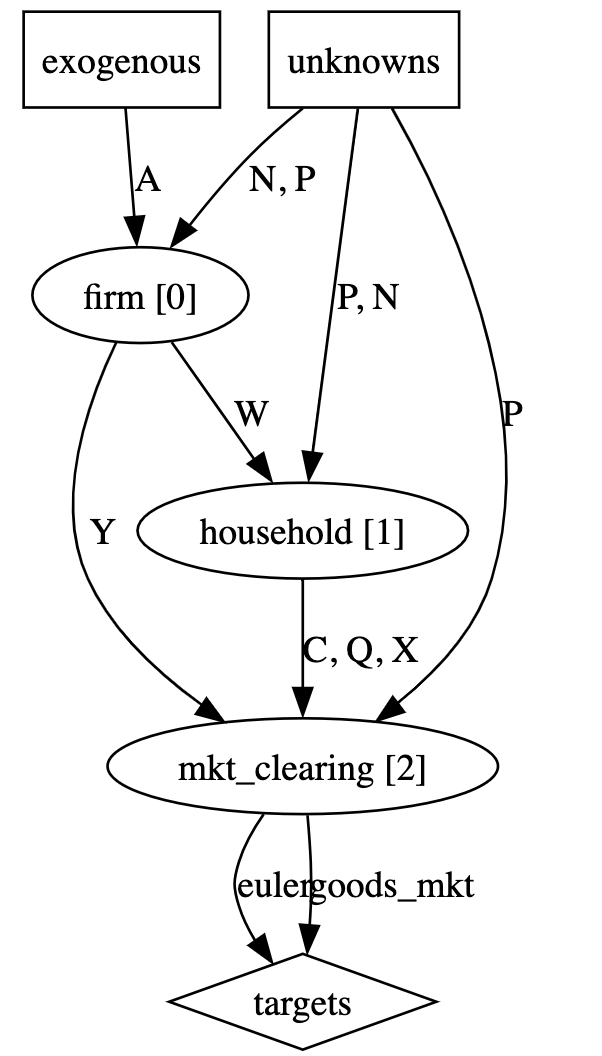
\includegraphics[width=0.3\textwidth]{figs/dag.png}
    \caption{DAG}
    \label{fig:dag}
\end{figure}

\begin{figure}[ht]
    \centering
    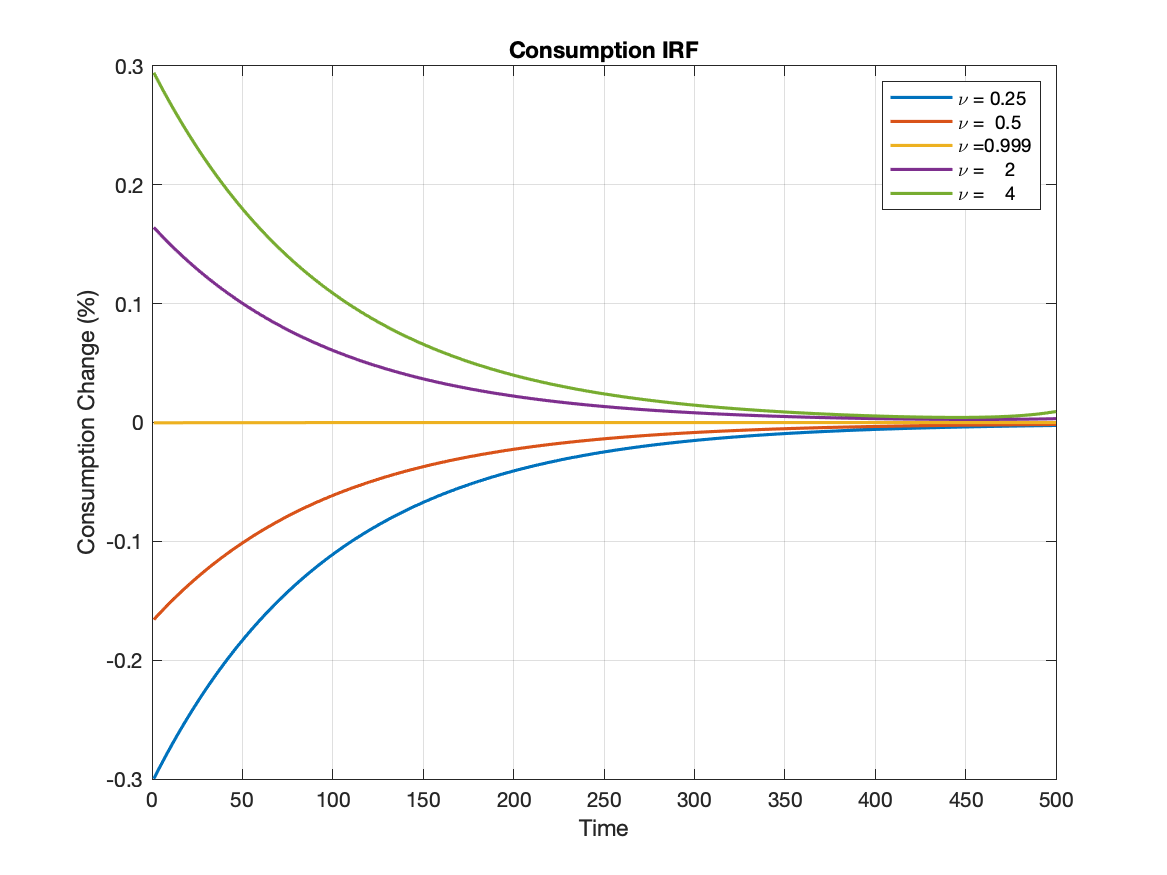
\includegraphics[width=0.4\textwidth]{figs/irf_c.png}
    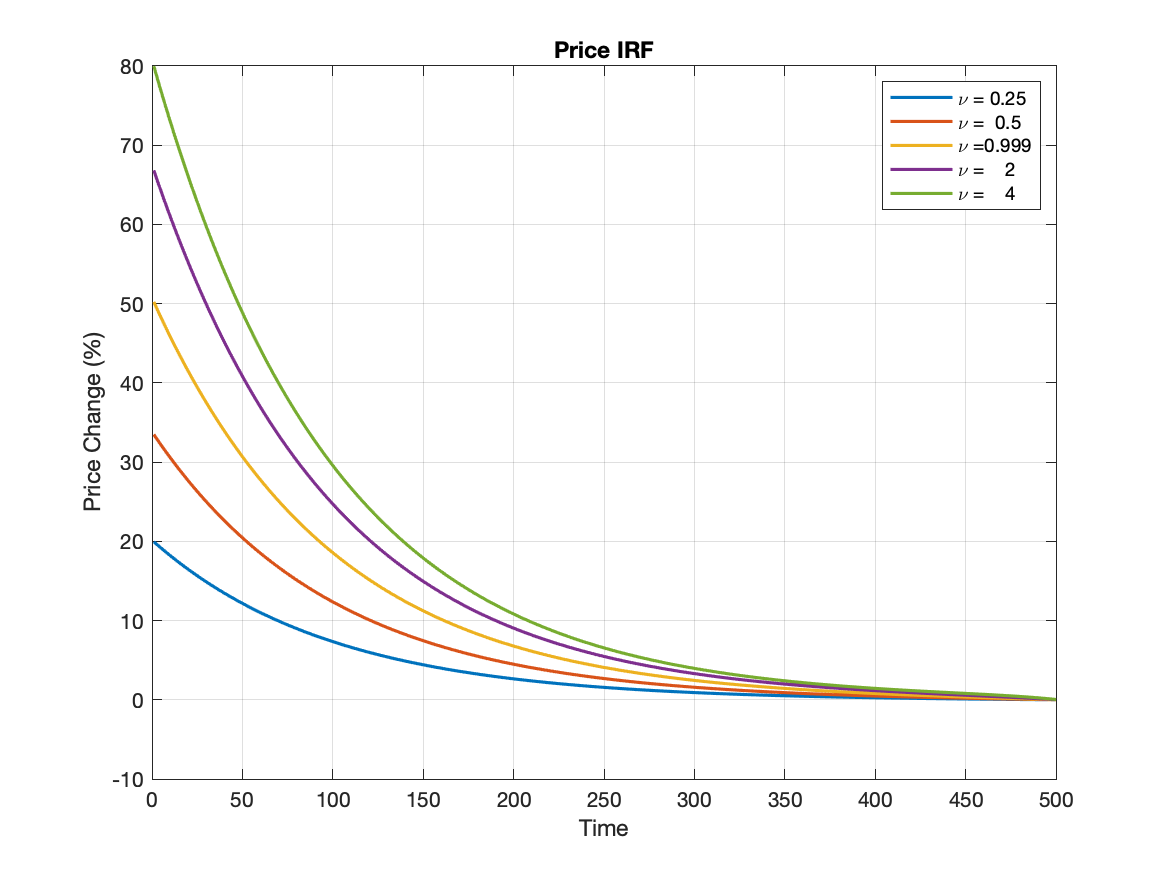
\includegraphics[width=0.4\textwidth]{figs/irf_p.png}
    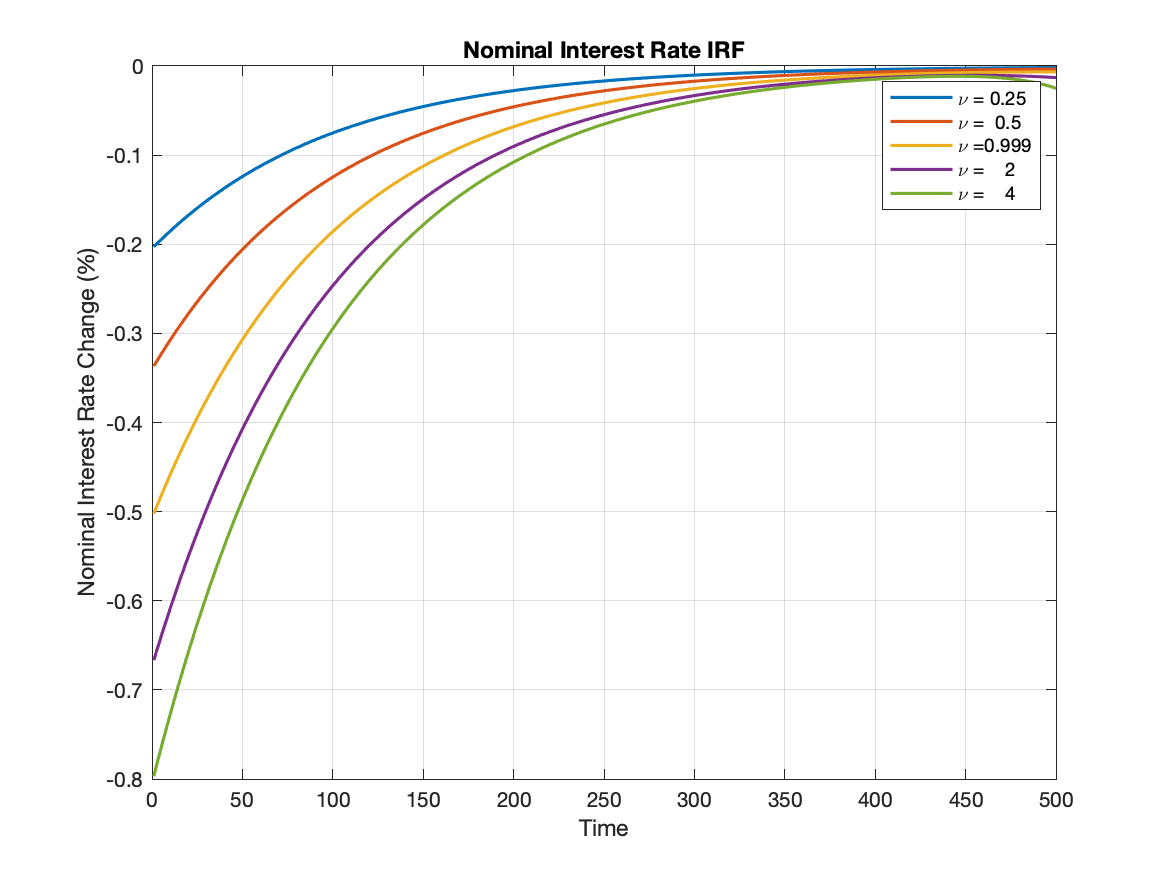
\includegraphics[width=0.4\textwidth]{figs/irf_q.png}
    \caption{Impulse responses for $C_t$, $P_t$ and $Q_t$}
    \label{fig:irf}
\end{figure}

Figure \ref{fig:dag} represents the DAG. 
Figure \ref{fig:irf} shows the impulse response functions of consumption, 
prices and norminal interest rate.

\section*{(i)}

$\nu$ is the reciprocal of the elasticity of substitution between consumption
and real balances. 
An increase in $\nu$ decreases the extent of an individual's trade-off between $C_t$ and $\frac{M_{t}}{P_{t}}$. 

When $\nu < 1$, the exponents of consumption and real balances in $X_{t}$ is positive, 
indicating that an increase in money supply decreases the marginal utility of consumption and labor supply. 
As a result, production and consumption diminish. 
When money supply goes up, the prices also go up. 
To support a hightened money demand, the interest rate declines. 

When $\nu = 1$, an increase in money supply does not change the marginal utility of consumption, 
so the household maintains their labor supply 
and production and consumption remain unchanged.  

When $\nu > 1$, the exponents of consumption and real balances in $X_{t}$ is negative. 
So, an increase in money supply leads to an increase in the marginal utility of consumption, 
compelling the household to supply more labor and subsequently boosts production and consumption. 
A higher $\nu$ also corresponds to an intertemporal substitution from money to consumption, 
resulting in higher prices and interest rates.

\section*{(j)}

Based on discussions in part (i), we need $\nu > 1$ to support the evidence 
that an increase in the money supply increases consumption.

\section*{(k)}

Please refer to \texttt{hw1\_sequence\_space.py}.


\end{document}

